\documentclass{sig-alternate-05-2015}

% *** CITATION PACKAGES ***
\usepackage{cite}

% *** MATH PACKAGES ***
\usepackage{amsmath}
\usepackage{svg}
\usepackage{amsfonts}
\usepackage{bm}

% *** PDF, URL AND HYPERLINK PACKAGES ***
\usepackage{url}
\usepackage{hyperref}
\usepackage{epigraph}

% *** ALGORITHM ***
%\usepackage{algorithm}
%\usepackage{algpseudocode}
\usepackage[ruled, linesnumbered]{algorithm2e}
\renewcommand{\algorithmcfname}{ALGORITHM}
\SetAlFnt{\small}
\SetAlCapFnt{\small}
\SetAlCapNameFnt{\small}
\SetAlCapHSkip{0pt}
\IncMargin{-\parindent}

\usepackage{booktabs}
\usepackage{enumitem}
\usepackage{float}

% *** To balance reference page ***
\usepackage[keeplastbox]{flushend}

% *** Draw diagrams ***
\usepackage{tikz}
\usetikzlibrary{positioning}
\usetikzlibrary{arrows.meta}

% *** Fancy Table ***
\usepackage{multirow}

\newcommand{\paragraphb}[1]{\vspace{0.03in}\noindent{\bf #1} }
\newcommand{\paragraphe}[1]{\vspace{0.03in}\noindent{\em #1} }
\newcommand{\paragraphbe}[1]{\vspace{0.03in}\noindent{\bf \em #1} }

\newcommand{\name}{DSSnet\xspace}
\newcommand{\Name}{DSSnet\xspace}

\newtheorem{lemma}{Lemma}
\newtheorem{theorem}{Theorem}
\newdef{definition}{Definition}

% *** For commenting blocks of text ***
\begin{document}

\CopyrightYear{2017} \setcopyright{acmcopyright}
\conferenceinfo{CS 558 Spring '17,}{March 10th, 2017, Chicago.}
\isbn{xxx-x-xxxx-xxxx-x/xx/xx}\acmPrice{\$15.00}
\doi{http://dx.doi.org/xx.xxxx/xxxxxxxxxx.xxxxxx}
%Authors, replace the red X's with your assigned DOI string.
\clubpenalty=10000
\widowpenalty = 10000

%
% --- Author Metadata here ---
%\conferenceinfo{WOODSTOCK}{'97 El Paso, Texas USA}
%\CopyrightYear{2007} % Allows default copyright year (20XX) to be over-ridden - IF NEED BE.
%\crdata{0-12345-67-8/90/01}  % Allows default copyright data (0-89791-88-6/97/05) to be over-ridden - IF NEED BE.
% --- End of Author Metadata ---

\title{A Comparative Study of Deep Learning Approaches in Off-Line Network Intrusion Detection
\titlenote{The codebase for our project is available on https://github.com/littlepretty/NetLearner}}

%
% You need the command \numberofauthors to handle the 'placement
% and alignment' of the authors beneath the title.
%
% For aesthetic reasons, we recommend 'three authors at a time'
% i.e. three 'name/affiliation blocks' be placed beneath the title.
%
% NOTE: You are NOT restricted in how many 'rows' of
% "name/affiliations" may appear. We just ask that you restrict
% the number of 'columns' to three.
%
% Because of the available 'opening page real-estate'
% we ask you to refrain from putting more than six authors
% (two rows with three columns) beneath the article title.
% More than six makes the first-page appear very cluttered indeed.
%
% Use the \alignauthor commands to handle the names
% and affiliations for an 'aesthetic maximum' of six authors.
% Add names, affiliations, addresses for
% the seventh etc. author(s) as the argument for the
% \additionalauthors command.
% These 'additional authors' will be output/set for you
% without further effort on your part as the last section in
% the body of your article BEFORE References or any Appendices.

\numberofauthors{2} %  in this sample file, there are a *total*
% of EIGHT authors. SIX appear on the 'first-page' (for formatting
% reasons) and the remaining two appear in the \additionalauthors section.
%

\author{
% You can go ahead and credit any number of authors here,
% e.g. one 'row of three' or two rows (consisting of one row of three
% and a second row of one, two or three).
%
% The command \alignauthor (no curly braces needed) should
% precede each author name, affiliation/snail-mail address and
% e-mail address. Additionally, tag each line of
% affiliation/address with \affaddr, and tag the
% e-mail address with \email.
%
% 1st. author
\alignauthor
Jiaqi Yan\\
\affaddr{Illinois Institute of Technology}\\
\affaddr{10 West 31st Street}\\
\affaddr{Chicago, Illinois, 60616 }\\
\email{jyan31@hawk.iit.edu}
% 2nd. author
\alignauthor
Dong Jin\\
\affaddr{Illinois Institute of Technology}\\
\affaddr{10 West 31st Street}\\
\affaddr{Chicago, Illinois, 60616 }\\
\email{dong.jin@iit.edu}
% 3rd. author
%\alignauthor
%Dong Jin\\
%\affaddr{Illinois Institute of Technology}\\
%\affaddr{10 West 31st Street}\\
%\affaddr{Chicago, Illinois, 60616 }\\
%\email{dong.jin@iit.edu}
%\and  % use '\and' if you need 'another row' of author names
%% 4th. author
%\alignauthor Lawrence P. Leipuner\\
%       \affaddr{Brookhaven Laboratories}\\
%       \affaddr{Brookhaven National Lab}\\
%       \affaddr{P.O. Box 5000}\\
%       \email{lleipuner@researchlabs.org}
%% 5th. author
%\alignauthor Sean Fogarty\\
%       \affaddr{NASA Ames Research Center}\\
%       \affaddr{Moffett Field}\\
%       \affaddr{California 94035}\\
%       \email{fogartys@amesres.org}
%% 6th. author
%\alignauthor Charles Palmer\\
%       \affaddr{Palmer Research Laboratories}\\
%       \affaddr{8600 Datapoint Drive}\\
%       \affaddr{San Antonio, Texas 78229}\\
%       \email{cpalmer@prl.com}
}



\maketitle
\begin{abstract}
Recently, a handful of novel deep neural networks have achieved unprecedentedly
good performance on image classification, natural language processing,
speech recognition and many other artificial intelligence related research fields.
In this project we investigate the possibility of applying the cutting edge
deep learning techniques to the network intrusion detection system.
We specifically look at a well-known public offline NSL-KDD network intrusion dataset and
compare the performance of several popular deep neural network architectures.
In this project, we
\begin{itemize}
    \item describe how we processing the NSL-KDD dataset so that
        it can be fed to deep neural networks;
    \item briefly introduce each deep neural network considered in this project;
    \item implement and train multi-layer percetron, restricted Boltzmann machine,
        sparse autoencoder and denoising autoencoder in TensorFlow;
    \item evaluate the classification performance in terms of accuracy, precision, recall as well as F1-Score.
\end{itemize}
The listed achievements above will serve as the basis in conducting
a comparative study of deep learning approaches in network intrusion detection.
\end{abstract}

%
%  Use this command to print the description
%
%\printccsdesc

% We no longer use \terms command
%\terms{Theory}

\keywords{Network Intrusion Detection System; Deep Learning}

\section{Introduction}

Network intrusion detection system (NIDS) is the essential security technology that
aims to protect any networked systems efficiently and automatically.
As either a hardware device or software application,
it monitors a network for malicious activities or policy violations.
By intercepting and analyzing the bi-direction traffics through the network,
it raises alarm if intrusion, attack or violation are observed.
There are two general approaches to detect intrusions.
In signature based intrusion detection, e.g. SNORT~\cite{Snort},
rules for specific attacks are pre-installed in the system.
It report suspicious traffic when the traffic matches any signature of known attacks.
The major drawback of signature matching approach is that
it is only effective for previously detected attacks that have an identifiable signature.
As a result, signature database needs to be manually updated whenever a new type of attack
is discovered, with significant effort, by the network administrator.
Anomaly detection based approach overcomes these limitations by adopting a certain
type of machine learning technique to model the trustworthy network activities.
Traffics that significantly deviates from the built model are treated as malicious.
This idea have been shown to be able to detect unknown or novel attacks~\cite{NSL-KDD, STL-NIDS}.
However, if the built model for normal traffics are not generalized enough,
anomaly based approach will treat unforeseen normal traffic as malicious,
suffering from high false positive.

In this project, we follow the anomaly detection based idea, and tries to enhance it with the
state-of-art machine learning technology, e.g. various deep neural networks trained by innovative algorithms.
Specifically, we have made the following contributions:
\begin{itemize}
    \item Firstly, we introduce the background of deep learning models and techniques,
        and discuss why they may better solve the network intrusion detection problem.
    %Besides, we also survey and discuss the status quo of available network intrusion detection datasets
    %and its implication on applying deep learning models to network intrusion detection.
    \item Then we briefly review the existing state-of-the-art machine learning solutions to network intrusion detection.
        After that, we describe several groups of the cutting-edge deep learning models
        in concisely mathematical languages.
    \item We conduct a quantitatively comparative study of each of them with
        two off-line network intrusion detection datasets~\cite{NSL-KDD, UNSW},
        with the help of our own TensorFlow-based deep learning library, NetLeaner.
        The detection performance is measured in accuracy, precision and recall.
    \item We not only make the codebase of NetLearner publicly available to research community,
        but also share the deep learning related hacks and tricks used during the training phase,
        so that future researches can easily reproduce and extend our work.
\end{itemize}


\section{Dataset and Preprocessing}
Among various available datasets~\cite{NSL-KDD, KDDCup, DARPA},
we choose NSL-KDD dataset~\cite{NSL-KDD} to evaluate the performance of applying
various deep neural networks to the network intrusion detection problem.
NSL-KDD dataset originates from the KDDCup 99 dataset~\cite{KDDCup},
which was used for the third International Knowledge Discovery and Data Mining Tool Competition.
However, NSL-KDD dataset addresses two issues of the KDDCup 99 dataset.
First, it eliminates the redundant records existing in KDDCup 99, which takes up
78\% and 75\% of the records in train and test set, respectively.
Second, it adds another label, classification difficulty, to each distinct record,
and samples the dataset such that the fraction of the record
from a difficulty level is inversely proportional to its difficulty.
Both enhancements make NSL-KDD dataset more suitable for
evaluation of intrusion detection systems.

The train dataset consists of 125,973 TCP connection records, while the test dataset
consists of 22,544 ones.
A record is defined by 41 features, including 9 basic features of individual
TCP connections, 13 content features within a connection and 9 temporal features computed
within a two-second time window, and 10 other features.
Connections in the train dataset are labeled as either normal or one of the 24 attack
types.
There are addtional 14 types of attacks in the test dataset, specifically designed to
test the classifier's ability to handle novel attacks.
The task of the classifier is to identify whether a connection is normal or one of the
4 categories of attacks, namely denial of service (DoS), remote to local (R2L), user to
root (U2R) and probing.
Alternatively, we can configure the classifier to report a connection to be either
normal or attack.
The former is called 5-class problem, whereas the later 2-class problem,
throughout this text.

Before feeding the NSL-KDD to neural networks, we need to take some preprocessing steps.
First and foremost, we need to convert symbolic features and the labels to one-hot encoding
format.
For example, if feature $f$ can take $n$ possible values from 1 to $n$,
feature value $x$ will be converted to a $n$-dimention binary vector with the $x$th
dimention set to 1 and others set to zero.
This can be done for the entire dataset (both train and test set)
using the \texttt{OneHotEncoder} provided by scikit-learn~\cite{OneHotEncoder}.
Then we shuffled the data, along with its label, so that later in the stochastic
gradient descent learning phase batch data are already randomized.
At last, we perform the min-max normalization so that data values are all in the range
of [0, 1].

\section{Deep Learning Architectures}
\label{Sec:Architectures}

In this section, we introduce a bunch of deep learning models that we consider promising in the
network intrusion detection problem.
For each architecture, we first give a brief mathematical introduction of it.
Then we describe how we build and train the model using a Python library NetLearner~\cite{NetLearner}.
NetLearner implements these deep learning models on the basis of TensorFlow.\footnote{TensorFlow~\cite{TensorFlow} is an open-source software library for machine learning developed by the Google Brain Team.}

\subsection{Multilayer Perceptron}
\label{SubSec:MLP}
Multilayer perceptron (MLP) is a classic deep learning classifier with simple
design of the connectivity between neurons.
It is a fully connected feed-forward neural network, as shown in Figure~\ref{Fig:MLPArchitecture}.
By introducing non-linear neural units (perceptrons), it can distinguish data that are
not linearly separable.
However, the non-linearity make it very hard to train a deep MLP of more than three layers,
even if people have proposed the efficient back-propagation learning algorithm~\cite{Backpropagation}.
Recently it revived due to the various new training techniques designed by deep learning community,
including Stochastic Gradient Descent (SGD), Adam optimizer~\cite{Adam},
batch normalization~\cite{BatchNorm} and Dropout~\cite{Dropout}.
Except for the number of neurons in each layer and number of layers,
MPL can also be tuned with different activation functions, or neural types.
The most popular two, which are used in this project, are logistic function
and rectifier linear unit.
Logistic function is written as
\begin{align}
    f(x) &= \frac{1}{1 + e^{-x}}
\end{align}
It has a very useful property when we applying back-propagation:
\begin{align}
    f'(x) &= f(x) (1-f(x))
\end{align}
Recently, most deep neural networks adopt rectifier neural unit and
achieved very good performance~\cite{DeepLearning}.
Rectifier linear unit is defined as
\begin{align}
    f(x) &= \max(0, x)
\end{align}
Let $\mathbf{a}^{(l)}$ be the activation of layer $l$,
$\mathbf{W}^{(l)}$ and $\mathbf{b}^{(l)}$ be layer $l$'s parameter.
With activation function defined, we have the following recursive formula that describes
the feed-forward step of the perceptron network.
\begin{align}
    \mathbf{z}^{(l+1)} &= \mathbf{W}^{(l)} \mathbf{a}^{(l)} + \mathbf{b}^{(l)} \label{Equ:MLPFeedForward1}\\
    \mathbf{a}^{(l+1)} &= f(\mathbf{z}^{(l+1)})
    \label{Equ:MLPFeedForward2}
\end{align}

\begin{figure}[h]
    \centering
    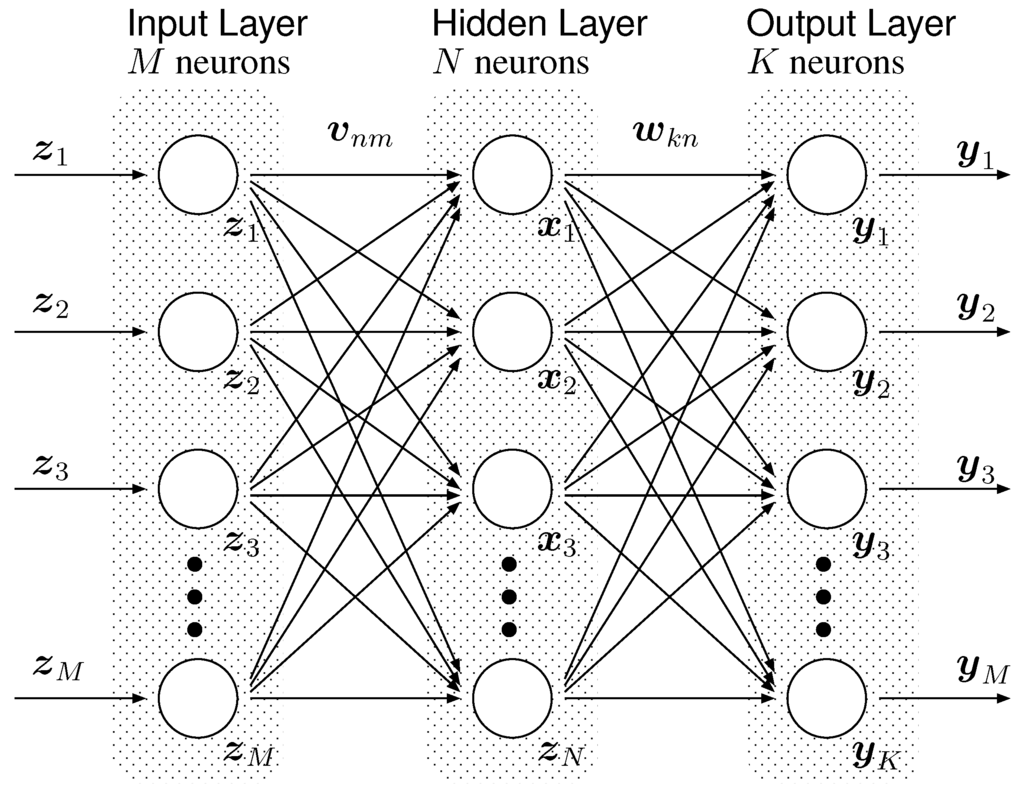
\includegraphics[width=0.45\textwidth]{figures/multilayer_perceptron.png}
    \caption{A multilayer perceptron neural network with 1 hidden layer.
        Figure courtesy of Teijiro Isokawa, Haruhiko Nishimura and Nobuyuki Matsui.}
    \label{Fig:MLPArchitecture}
\end{figure}

We build two dual-hidden-layer MLP, with 800 neurons in first layer,
and 480 neurons in the second layer followed by a softmax classifier,
one for the NSL-KDD task and the other for the UNSW-NB15 task.
Both MLP are trained with Adam optimizer~\cite{Adam} for 200 epochs and batch size 80.
During the training, learning rate decays from 0.1 exponentially with the base of 0.96.
We do not include regularization in the model, but do apply dropout of probability 0.2.
We denote both MLP models as MLP and show their detailed results in the later section.

\subsection{Restricted Boltzmann Machine}
Restricted Boltzmann machine (RBM)~\cite{RBMTechReport} is a type of energy-based model,
which associate a scalar energy to each configuration vector of the variables in the network.
In energy-based model, learning is the process of configuring the network weights so that
the average energy over training data is minimized.
RBM consists of a layer of hidden units (H) and a layer of visible units (V).
Here ``restricted" means that connections are just between hidden and visible layer,
but not within hidden layers or visible layers.
This makes its training to be faster than Boltzmann machine and makes it feasible to
stack multiple separately trained RBM together to form deep architecture.
A joint configuration, $(\mathbf{v, h})$, of the visible and hidden units has the energy of
\begin{align}
    E(\mathbf{v, h}) &= -\sum_{i\in visible}a_i v_i - \sum_{j\in hidden}b_j h_j - \sum_{i, j}v_i h_j w_{ij}
\end{align}
where $a=\{a_i\}$ and $b=\{b_j\}$ are biases in visible and hidden layer respectively,
and $W=\{w_{ij}\}$ is the weights between them.
The network assigns a probability to every possible pair of $(\mathbf{v, h})$ via this energy
function
\begin{align}
    p(\mathbf{v, h}) &= \frac{1}{Z} e^{-E(\mathbf{v, h})} \\
    p(\mathbf{v}) &= \frac{1}{Z} \sum_{\mathbf{h}} e^{-E(\mathbf{v, h})}
\end{align}
where $Z$ is the partition function that equals to the summation over all possible hidden
and visible vector pairs
\begin{align}
    Z = \sum_{\mathbf{v,h}} e^{-E(\mathbf{v, h})}
\end{align}
Based on the ``maximizing log likelihood" idea,
we want to raise the probability of a training example and it can be done by
adjusting the weights biases to lower the energy of the considered example.
Meanwhile, we can let other examples make a big contribution to the partition function $Z$
by raising their energy.
Both insights can be translated to the following formula:
\begin{align}
    \frac{\partial \log p(v)}{\partial w_{ij}} = \langle v_i h_j \rangle_{data} - \langle v_i h_j \rangle_{model} 
\end{align}
This implies the following learning rule for performing stochastic gradient ascent on training
data
\begin{align}
    \Delta w_{ij} &= \varepsilon (\langle v_i h_j \rangle_{data} - \langle v_i h_j \rangle_{model})
\end{align}
The first term $\langle v_i h_j \rangle_{data}$ is the sampling from the data and it is easy to
compute since there is no directed connection between hidden units.
The sampling of $h_j$ is based on the probability
\begin{align}
    Prob(h_j = 1 | \mathbf{v}) &= sigmoid(b_j + \sum_i{v_i w_{ij}})
    \label{Equ:RBMSampleHidden}
\end{align}
Similarly, $v_i$ can be sampled with the following distribution
\begin{align}
    Prob(v_i = 1 | \mathbf{h}) &= sigmoid(a_j + \sum_j{h_i w_{ij}})
    \label{Equ:RBMSampleVisible}
\end{align}
The term $\langle v_i h_j \rangle_{model}$ can be obtained by performing alternative Gibbs
sampling for a long time.
The sampling starts from a random visible state.
Then we update the hidden units in parallel with Equation~\ref{Equ:RBMSampleHidden},
followed by updating the visible units in parallel with Equation~\ref{Equ:RBMSampleVisible}.
Instead of doing alternating Gibbs sampling for a large number of iterations,
\cite{TrainCD} proposed contrastive divergence (CD) as a faster learning procedure.
The training also start with a training vector to compute the states of the hidden units
using Equation~\ref{Equ:RBMSampleHidden}.
Then, with the chosen hidden states, we reconstruct the visible states by sampling each $v_i$
with probability given in Equation~\ref{Equ:RBMSampleVisible}.
The change of weight is then computed by
\begin{align}
    \Delta w_{ij} = \varepsilon (\langle v_i h_j \rangle_{data} -
    \langle v_i h_j \rangle_{reconstruct})
    \label{Equ:RBMCD1}
\end{align}
This is called contrastive divergence using one full step of alternating Gibbs sampling.
Contrastive divergence with $n$ rounds of alternating Gibbs sampling
is usually denoted as CD$n$.

For each task, we build a RBM with 800-hidden units to perform unsupervised learning first on the dataset.
We train the RBM using CD1 with batch size 10 for 160 epochs.
The learning rate is initialized at 0.01 and decay exponentially with the base of 0.64.
We then create a separate MLP with the same configuration as in section~\ref{SubSec:MLP},
and initialize its weights of the first hidden layer (also 800 neurons) to be that of the RBM's.
We hope such action could enhance the quality of MLP.
Then we finetune the MLP for 300 epochs with small learning rate of 0.01.
We denote this restricted Boltzmann machine initialized MLP as RBM and report its
performance in the later section.

\begin{figure}[h]
    \centering
    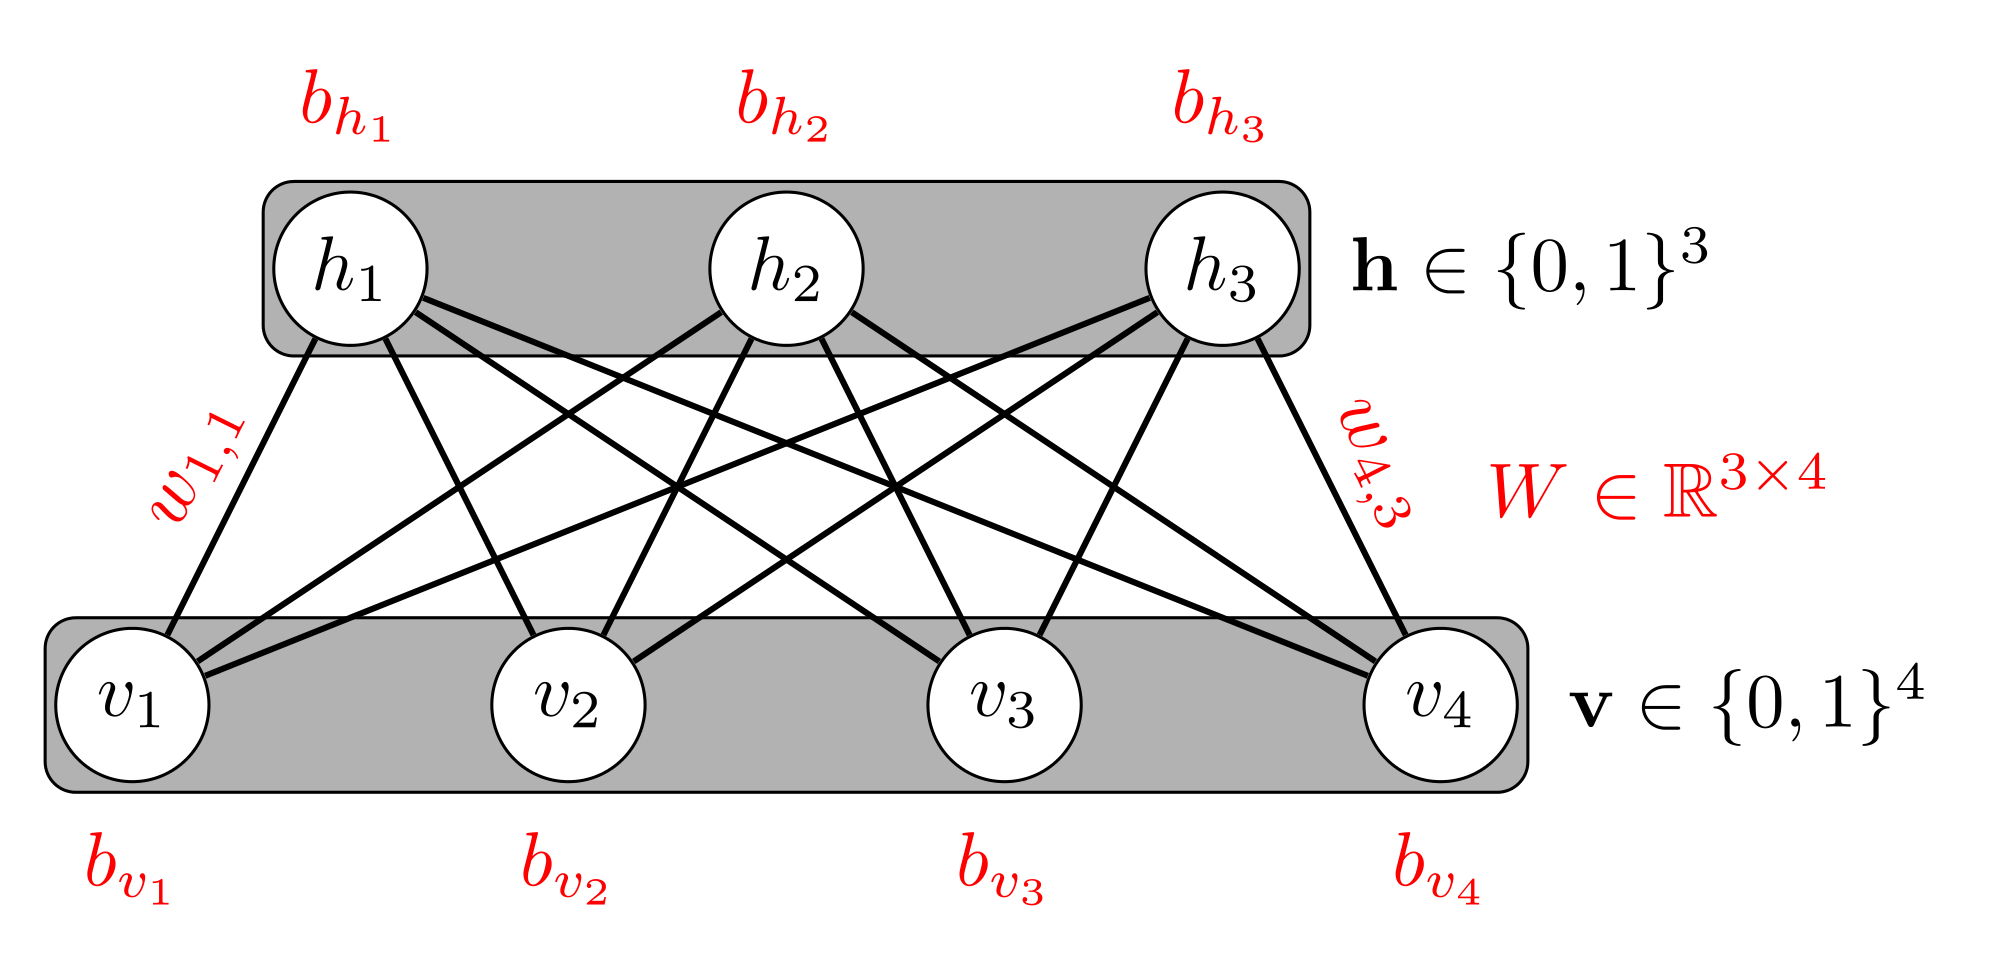
\includegraphics[width=0.45\textwidth]{figures/rbm.png}
    \caption{Restricted Boltzmann Machine.
        Figure courtesy of https://commons.wikimedia.org/wiki/File:Restricted-boltzmann-machine.svg}
    \label{Fig:RBMArchitecture}
\end{figure}


\subsection{Autoencoders}
An autoencoder neural network is an unsupervised model with typically one hidden layer that
tries to set the output layer to be equal to the input.
As shown in Figure~\ref{Fig:AEArchitecture}, we want the network to
learn a function $h_{W, b}(x) \approx x$.
However, to prevent the network from learning the meaningless identity function,
we need to place extra constraints on the network, giving birth to different
flavors of autoencoders.
In this project we consider one of the most popular types of autoencoder, sparse autoencoder.

\begin{figure}[h]
    \centering
    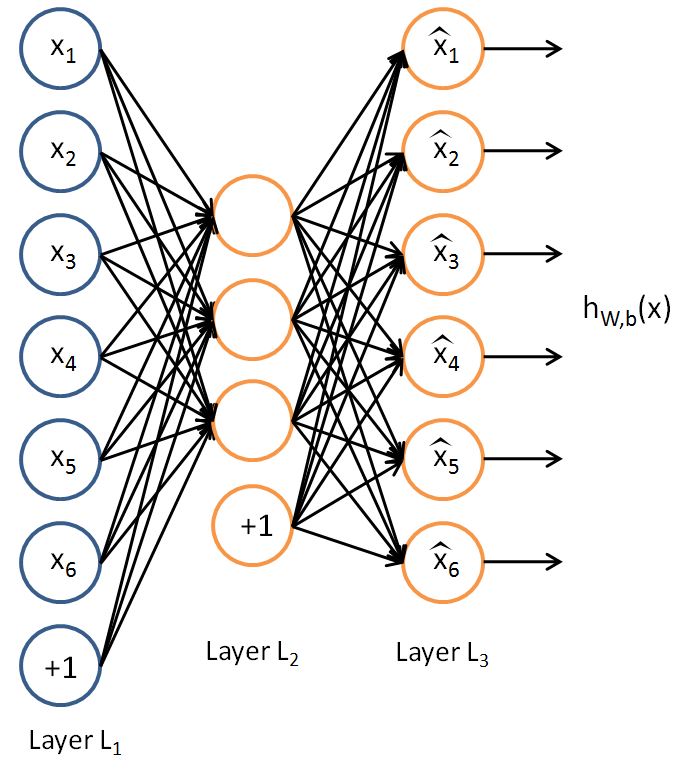
\includegraphics[width=0.45\textwidth]{figures/autoencoder.png}
    \caption{General Architecture of Autoencoders.
        Figure courtesy of~\cite{UFLDLAutoencoder}.}
    \label{Fig:AEArchitecture}
\end{figure}

\iffalse
The \textbf{denoising autoencoder} algorithm is proposed by~\cite{DenoiseAE} and illustrated in
Figure~\ref{Fig:dAEAlgorithm}.
To prevent learning identity function, an example $\mathbf{x}$ is first corrupted, either by
adding Gaussian noise or by random masking a fraction of items in $\mathbf{x}$ to zero.
The autoencoder then maps corrupted $\mathbf{\tilde{x}}$ to a hidden representation $\mathbf{y} = sigmoid(\mathbf{W}\tilde{\mathbf{x}} + \mathbf{b})$.
From $\mathbf{y}$ we reconstruct $\mathbf{z}=g_\theta'(\mathbf{y})$.
The training needs to learn the parameters $\theta$ and $\theta'$ so that
average reconstruction error is minimized over training set.
For binary input $\mathbf{x}$, usually cross entropy is adopted as $L_H(\mathbf{x}, \mathbf{z})$;
while mean squared error is used for real-valued $\mathbf{x}$.

Denoising autoencoder and sparse autoencoder, surprisingly, have different application domains.
Vincent et al.~\cite{DenoiseAE} have shown that stacked denoising autoencoder can be used to
initialize a deep neural network's weight parameter,
achieving similar and sometimes better performance than stacked RBM.
They also show that training stacked denoising autoencoder with MNIST dataset, it is able
to re-synthesize a variety of similarly good quality digits.
Raina et al.~\cite{SparseAE} have compared sparse encoding with principle component analysis
(PCA) and argue that transferring raw features with a well unsupervised trained
sparse autoencoder can be beneficial to supervised learning algorithms,
for example support vector machines (SVM).
\begin{figure}[h]
    \centering
    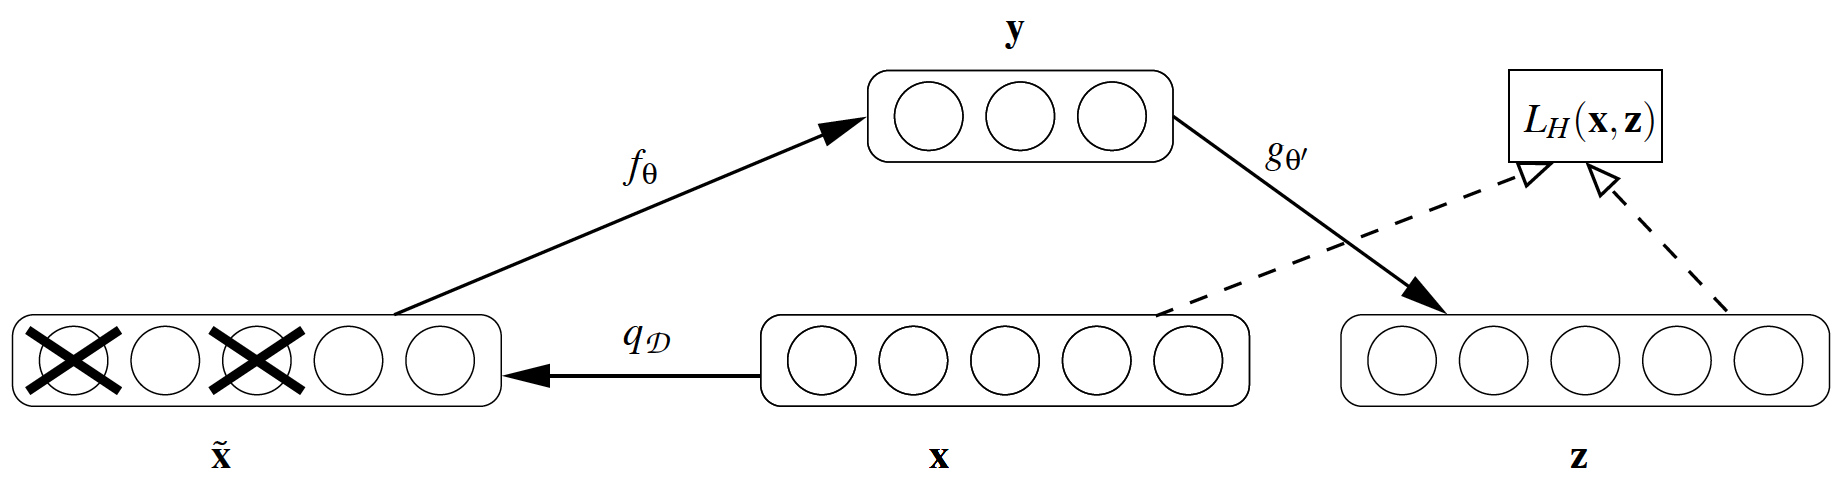
\includegraphics[width=0.45\textwidth]{figures/denoiseautoencoder.png}
        \caption{The denoising autoencoder algorithm.
        Input example $\mathbf{x}$ is randomly corrupted via $q_\mathcal{D}$ and then
        is mapped via encoder $f_\theta$ to $\mathbf{y}$.
        The decoder $g_\theta'$ attempts to reconstruct $\mathbf{x}$ and produces $\mathbf{z}$.
        Reconstruction error is measured by loss $L_H(\mathbf{x}, \mathbf{z})$, to be minimized
        during the training phase.
        Figure courtesy of~\cite{DenoiseAE}.}
    \label{Fig:dAEAlgorithm}
\end{figure}

\fi

The \textbf{sparse autoencoder} works by placing a sparsity constraint on the hidden units~\cite{SparseAE}.
First, we make the autoencoder's hidden layer size to be over-complete,
that is, of larger size comparing to the dimension of the input.
Let's denote the activation of hidden unit $j$ of layer 2 in Figure~\ref{Fig:AEArchitecture}
to be $a^2_j(\mathbf{x})$ given input example $\mathbf{x}$.
With that, we define the average activation of hidden unit $j$ over the $m$-size
training set
\begin{align}
    \hat{\rho}_j = \frac{1}{m} \sum_{i=1}^{m} a^2_j(\mathbf{x})
\end{align}
The sparsity constraint is enforcing, $\forall$ hidden unit $j$,
\begin{align}
    \hat{\rho}_j = \rho
\end{align}
where $\rho$ is a sparsity parameter that approximates zero (say 0.05).
This constraint can be vectorized over the hidden layer, say of size $n_2$,
with the KL divergence based penalty term
\begin{align}
    \sum_j^{n_2} KL(\rho || \hat{\rho}_j)
    = \sum_j^{n_2} [\rho \log \frac{\rho}{\hat{\rho}_j} + (1 - \rho) \log \frac{1-\rho}{1-\hat{\rho}_j} ]
\end{align}
The sparsity penalty term is integrated into the cost function by adding another hyper-parameter $\beta$
\begin{align}
    L(W, b) = \frac{1}{2}||h_{W,b}(\mathbf{x}) - \mathbf{x}||^2 +
    \beta \sum_j^{n_2} KL(\rho || \hat{\rho}_j)
\end{align}

Our implementation of the sparse autoencoder is different from the
self-taught learning approaches in~\cite{STL-NIDS, SparseAE},
which also adopting sparse autoencoder as the unsupervised feature learner.
In their work, the hidden features learnt by sparse autoencoders are used directly by
a classifier, for example, a softmax regressor or a SVM.
The functionality of autoencoder resembles a transformation of raw dataset
by approaches such as principle component analysis,
aiming to obtain a new feature space beneficial to general supervised learning algorithms.

Our way of utilizing autoencoder is to initialize the first layer weights of a MLP,
similar to how we use RBM.
The over-complete hidden layer size of the sparse autoencoder is 800;
the sparsity value $\rho$ is 0.05.
The autoencoder is trained with ADADELTA~\cite{ADADELTA} for 200 epochs and batch size 80.
We then create a separate MLP with same configuration as that in section~\ref{SubSec:MLP}
and initialize its first layer weights with the learnt weights of the autoencoder.
During finetuning the MLP, we used SGD optimizer with very small initial learning rate 0.004
and decaying 1e-6 over each update.
We denote this approach as SAE and report its performance in the later section.


\iffalse
\subsection{Generative Adversarial Nets}
As another generative model, Generative Adversarial Nets (GAN)\cite{GAN} adopts a novel training framework,
in which two models are trained simultaneously and adversarially.
The generative model $G(z;\theta_g)$ aims to capture the probability distribution of the available unlabelled dataset,
where its input is a noise variable $z$ following a prior distribution $p_z$.
The discriminative model $D(x;\theta_d)$ output the probability distribution that whether the its input source $S$ comes
from training dataset ($x\sim data$) or the generative model ($x \sim G(z)$):
\begin{align}
    D(X) = P(S|X)
\end{align}

Models $G$ and $D$ can be as simple as multilayer perceptrons,
or as complex as deep convolutional nets when the task domain is image.
The two models are trained in opposition to one another, with respect to the following log-likelihood function

\begin{align}
V(D, G) & = \mathbb{E}_{\bm{x}\sim data} [\log P(S=real|X=\bm{x})] + \mathbb{E}_{\bm{x}\sim G(\bm{z})} [\log P(S=fake|X=\bm{x})] \\
        & = \mathbb{E}[\log D(\bm{x})] + \mathbb{E}[\log (1 - D(G(\bm{z})))]
\end{align}

With $V(D, G)$ properly defined, the training procedure is a two-player minimax game.
First we maximize the log-likelihood that $D$ correctly recognize
both the training examples and the samples generated from $G$;
in the following phase, we train $G$ to generate samples that trick $D$ to make most mistakes.
This two-phase min-max optimization can be summarized as:
\begin{align}
    \min_G \max_D V(D, G)
\end{align}

Powerful though GAN is, large amount of efforts and care are needed during training.
One way to make the training stable and fast is to augment GAN with an auxiliary classifier so that
the training phase employs the labels available in the dataset~\cite{AC-GAN}.
In auxiliary classifier GAN (AC-GAN), the discriminator $D$ now gives both the probability
distribution over the sources (whether $\bm{x}$ is real or fake) and the probability distribution
over the class labels:
\begin{align}
    D(X) = P(S|X), P(C|X)
\end{align}
Accordingly, the log-likelihood function $V(D, G)$ is augmented with the log-likelihood of the correct class $L_C$:

\begin{align} 
    V(D, G) &= L_S + L_C \\
    L_S &= \mathbb{E}_{\bm{x} \sim data} [\log P(S=real|X=\bm{x})] + 
    \mathbb{E}_{\bm{x} \sim G(\bm{z})} [\log P(S=fake|X=\bm{x})] \\
    L_C &= \mathbb{E}_{\bm{x} \sim data}[\log P(C=c|X=\bm{x})] + 
    \mathbb{E}_{\bm{x} \sim G(\bm{z})} [\log P(C=c|X=\bm{x})]
\end{align}

The training procedure for AC-GAN is similar to GAN: we train $D$ to maximize $V(D, G)$;
while at the same time we train $G$ to minimize $L_S - L_C$.
Currently, we are interested in using GAN or AC-GAN to generate fake traffic.
In the future, we will also attempt the semi-supervised classification framework with AC-GAN.
\fi

\subsection{Wide and Deep Learning with Embeddings}
\label{SubSec:WD}
In the network intrusion dataset, categorical and integer features are extremely sparse.
For illustration reason, we plot the histogram of the ``dloss" integer feature in UNSW-NB15 dataset,
which denotes the number of destination packets retransmitted or dropped.
As shown in~\ref{Fig:DlossHist}, ``dloss"'s values range from 0 to 6000, while more than 97\%
of the occurred value is 0 but values from 1000 to 6000 do appear in the dataset.
For categorical feature ``proto", which tells one of the 133 protocol types the traffic record belongs to,
one-hot encoding it will make it become a 133-dimension vector with only one field being one.
Usually neural networks are not good at utilizing sparse large dimension input.

We tackle this problematic situation in two ways,
resulting in the combined model proposed in~\cite{WideDeepModel}.
The first solution is to embed the integer or categorical features.
Simply put, an embedding is a mapping from sparse discrete objects to a dense vector of real numbers.
It is widely used, also known as ``word2vec", in the natural language processing and machine translation tasks,
where embeddings are treated as points in vector space such that similarity between objects can be visually measured
by the Euclidean distance or angle between vectors.
In our case, embedding provide a solution to converting large-vocabulary-size categorical features
and sparse integer features to dense vectors of continuous values.
Deep neural network fed with embedding inputs can generalize better even with less feature engineering.
As stated in~\cite{WideDeepModel}, these input features to the deep neural nets are denoted as deep components,
consisted of continuous, one-hot encoded, and embedded features.

On the other hand, we leverage simple linear models with nonlinear feature transformations to deal with sparse inputs,
namely the wide components proposed in~\cite{WideDeepModel}.
The wide components consist of two parts: the basis and crossed features.
The basis features are raw input features that are either integer or categorical.
The crossed features are cross-product transformations of basis features:
\begin{align}
    \Phi_k (\bm{x} ) = \prod_{i=1}^{d} {x_i}^{c_{ki}}
\end{align}
where
\begin{align}
    c_{ki} = 
    \begin{cases}
        1, & \text{$i$-th feature $\in$ the transformation $\Phi_k$} \\
        0, & \text{otherwise}
    \end{cases}
\end{align}

\begin{align}
    \Phi_k (\mathbf{x} ) = \prod_{i=1}^{d} {x_i}^{c_{ki}}, \text{ where }
c_{ki} = 
\begin{cases}
    1, & \text{$i$-th feature $\in \Phi_k$} \\
    0, & \text{otherwise}
\end{cases}
\end{align}
The function of wide components, especially the cross-product transformations,
is memoization of the raw feature interactions.

In summary, the Wide and Deep model actually complements a deep neural network
with embedded low-dimension input vectors for good generalization;
Its linear sub-model, as shown in Figure~\ref{Fig:WideDeepModel}, is integrated with the deep neural network using a weighted sum of each model's output for good memorization.

The wide and deep learning model requires engineering the raw attributes in dataset into basis, crossed, continuous, and embedded components.
In our implementation, the basis features are all the raw symbolic and integer attributes.
Crossed features are built by a subset of combinations of the symbolic attributes in a dataset.
The raw symbolic and integer attributes are fed to the deep neural network as embedded components after conducting embedding.
The continuous components are straitforwardly the raw continuous attributes.
To compare with previous proposed models, we set the structure of the deep neural network in the wide and deep model to be
the same sizes as that of the baseline MLP, namely two hidden layers with size of [800 480].

\begin{figure}[h]
    \centering
    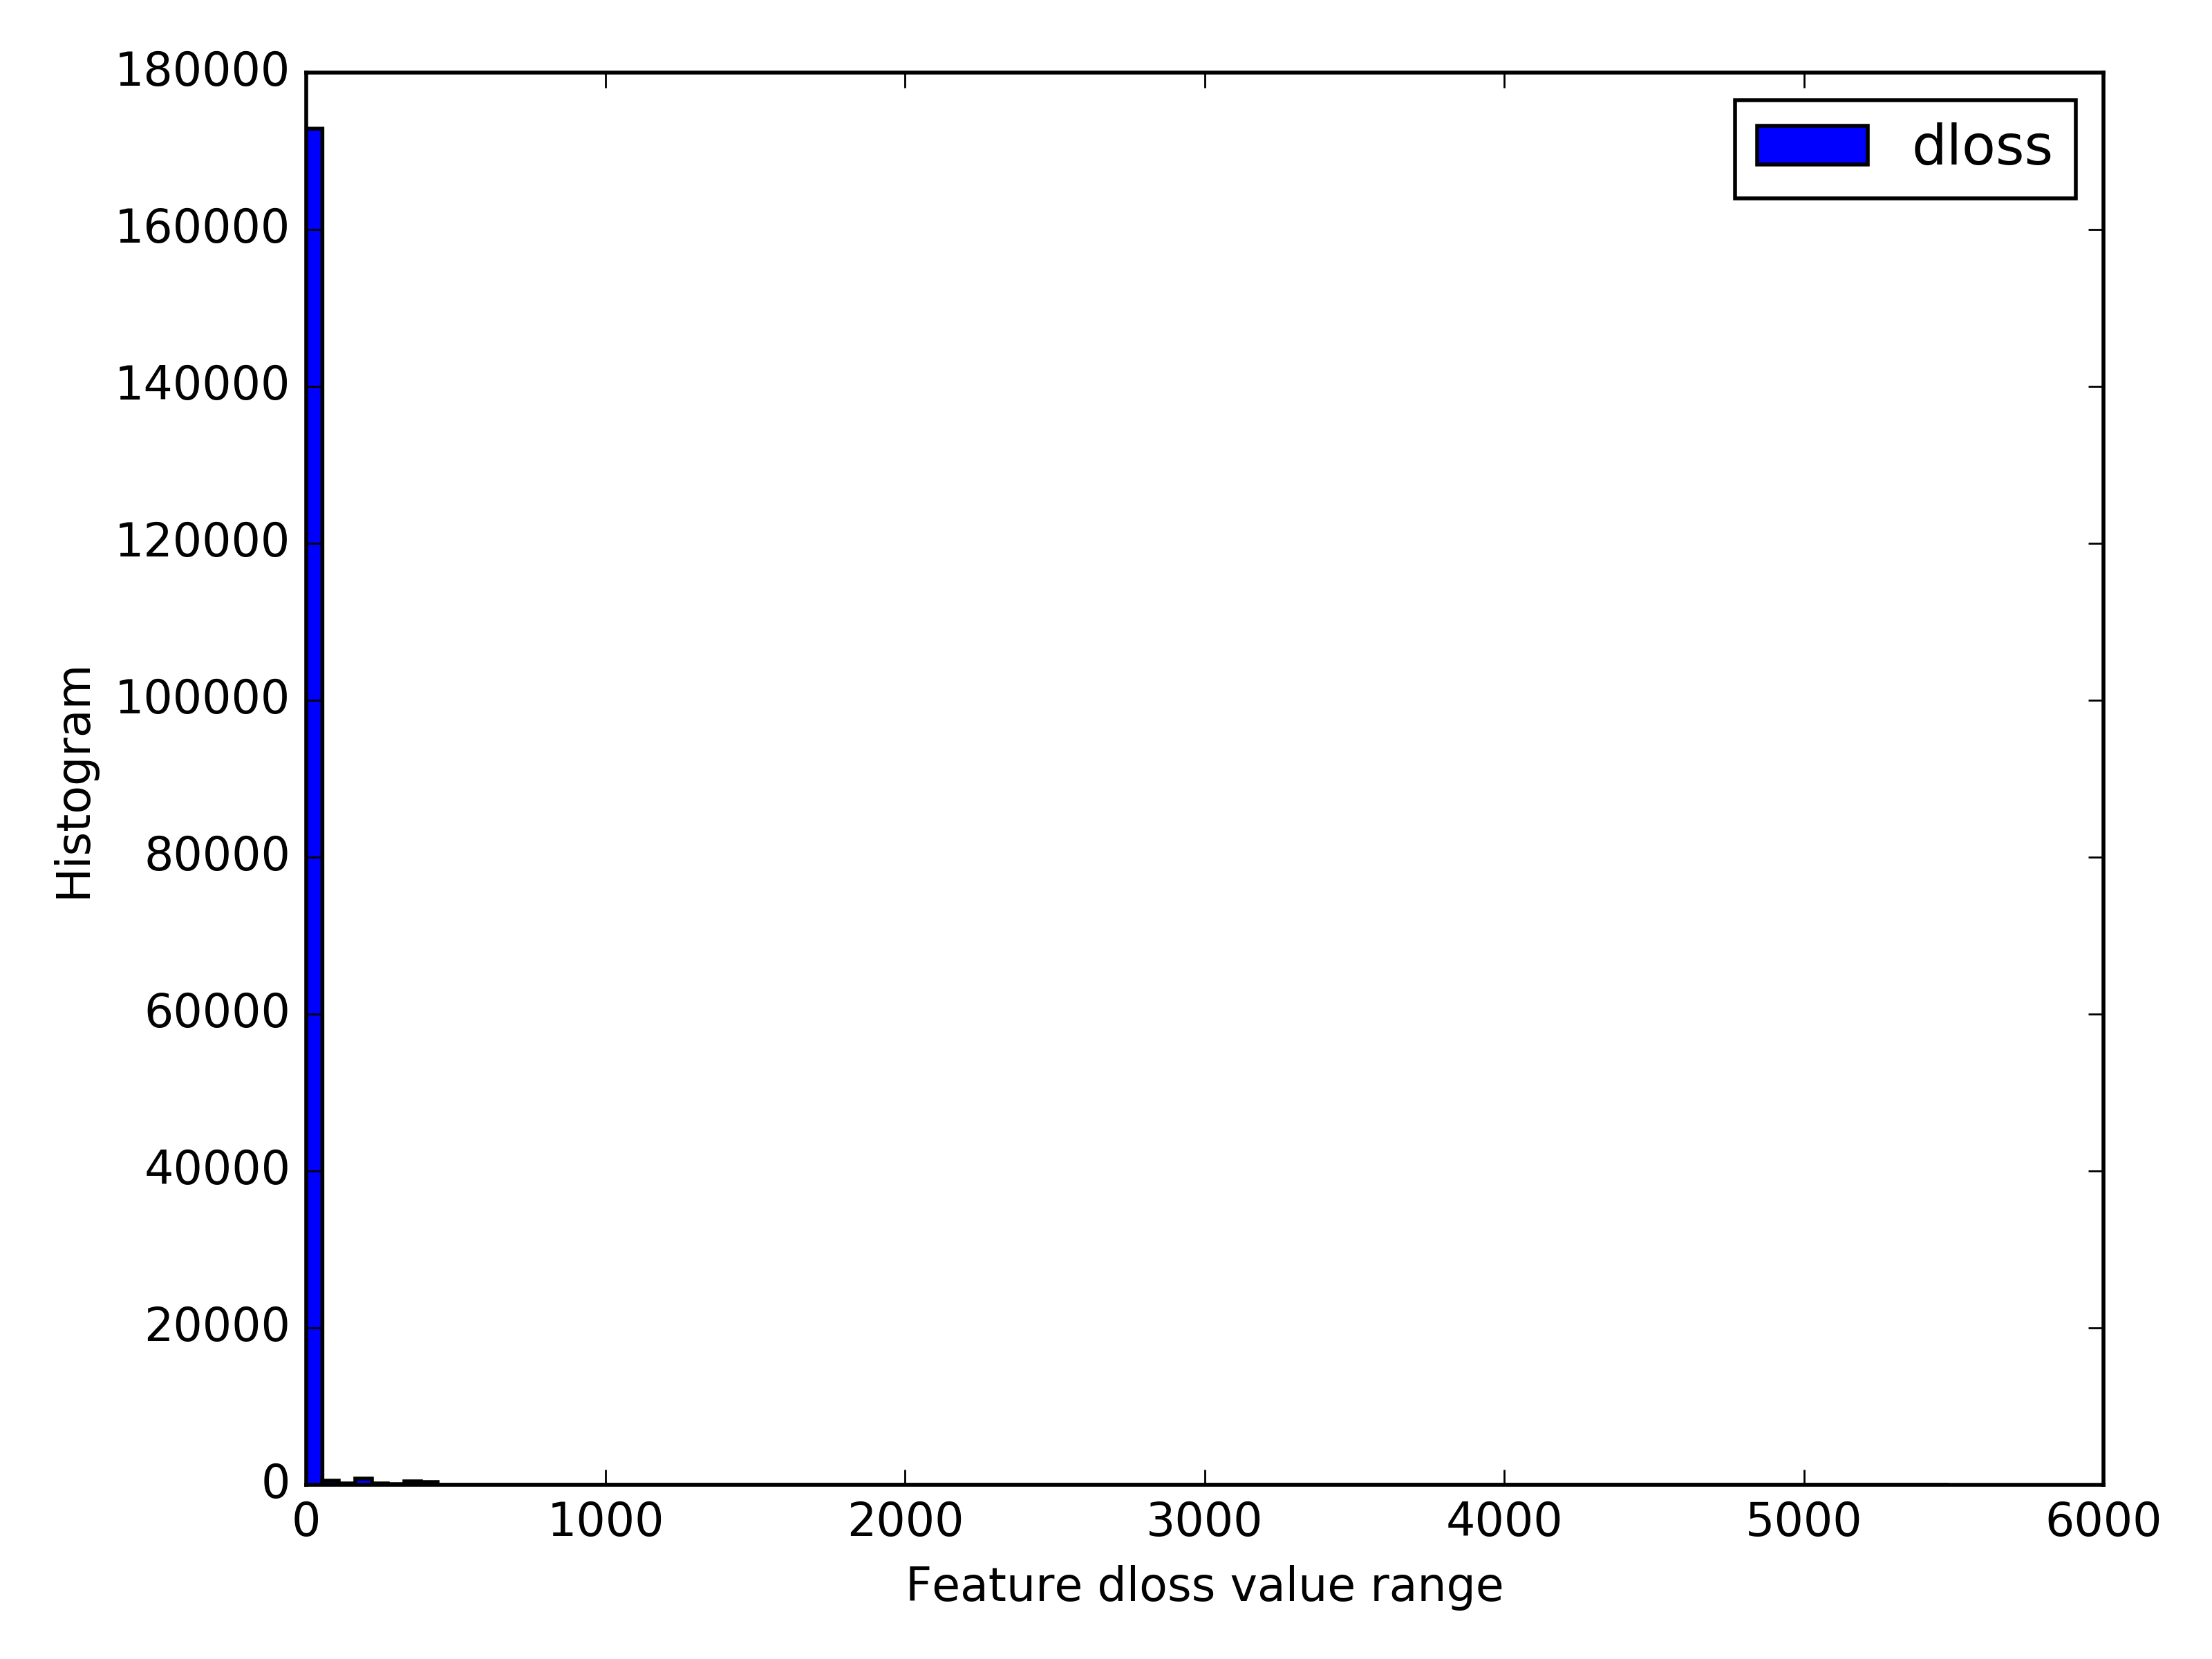
\includegraphics[width=0.45\textwidth]{figures/dloss_hist.png}
    \caption{Histogram of the Feature ``dloss" from UNSW-NB15 Dataset.}
    \label{Fig:DlossHist}
\end{figure}

\begin{figure*}[h]
    \centering
    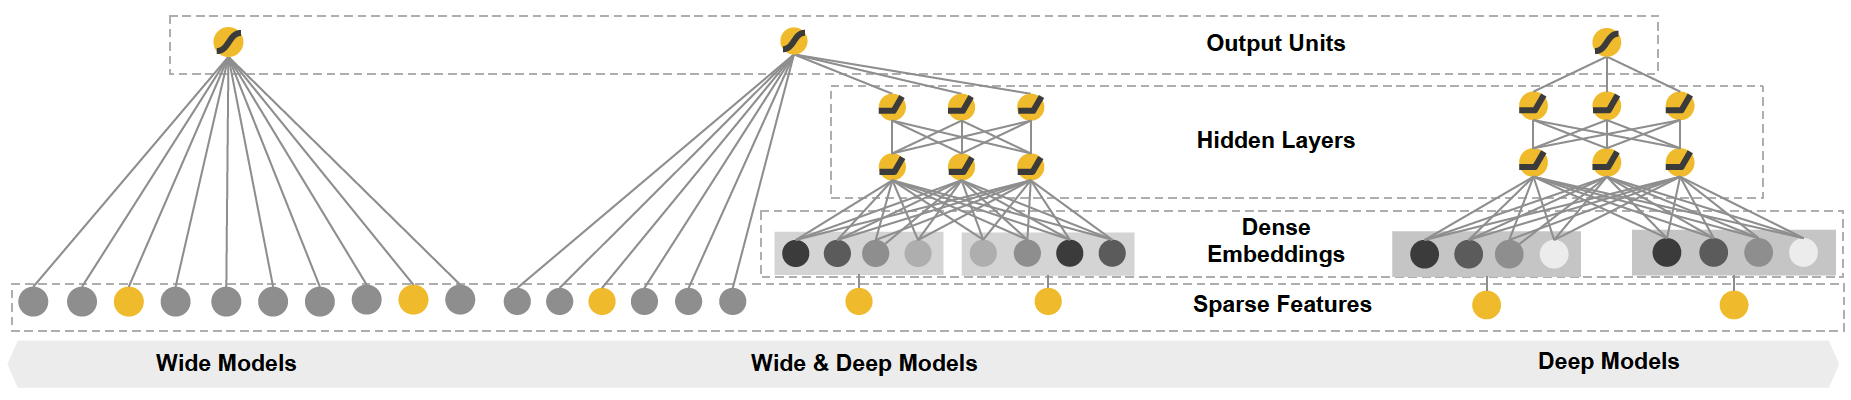
\includegraphics[width=0.98\textwidth]{figures/WideDeepModel.png}
    \caption{Anatomy of Wide and Deep Model}
    \label{Fig:WideDeepModel}
\end{figure*}

\section{NetLearner}

\iffalse
\subsection{TensorFlow 101}
The library models the computations in machine learning as data flow graphs.
Multidimensional data arrays are called tensors in TensorFlow.
Nodes in the graph represent mathematical operations between tensors,
such as add, multiply, softmax and dropout.
Graph edges represent the flow of tensors between nodes.
The computation graph based architecture allow researchers to run or train neural networks
on one or more CPUs or GPUs with unified API.

For general classification task, input $X$ and label $Y$ are defined as \textbf{placeholder}s
and feed into the computation graph at running time using a dictionary.
The graph of a typical deep learning model have three parts.
The \textbf{inference} graph should be built so that output predictions are returned as tensor.
For example, in the multilayer perceptron case, inference graph contains all iterative
computation~\ref{Equ:MLPFeedForward1}-\ref{Equ:MLPFeedForward2} in the feed-forwarding steps.
The \textbf{loss} graph should compute the loss function defined by specific models or algorithms.
Usually it is either cross-entropy or mean-squared error averaged across the batch data.
The loss graph will be optimized, usually minimized, by the \textbf{train} part.
This optimization can be conducted by various optimizing algorithms, such as gradient descent,
Momentum, RMSProp.
After sufficient steps of batch training, we evaluate the trained model with inference
graph and compare the predictions with the test dataset labels.
TensorFlow also provides various useful utilities for training models and running experiments.
Using a Saver, we are able to checkpoint the training process so as to restoring the model
for further training or evaluation.
Users create Summary nodes to log the snapshot of interest variables, which can be
automatically visualized by TensorBoard.
\fi

We provide a Python library NetLearner~\cite{NetLearner} that wraps up several deep learning models on the basis of TensorFlow.
TensorFlow~\cite{TensorFlow} is an open-source software library for machine learning
developed by the Google Brain Team.
NetLearner modularizes multilayer perceptron, restricted Boltzmann machine, and autoencoders.
We utilize NetLearner to perform the 5-class classification on the NSL-KDD dataset and 2-classification on the UNSW-NB15 dataset

\subsection{Training Support Vector Machines}

\subsection{Training Multilayer Perceptron}
For the multiple layer perceptron, we tried a 4-hidden-layer network with
very wide size in each layer, several hundreds for each layer.
The accuracy on training set is very exiting, usually more than 96\%.
However, its performance on test dataset is not satisfactory.
Instead we found out that a single hidden layer with only sixteen neurons has good accuracy.
It is trained with stochastic gradient descent (SGD) for 20 epochs and batch size 100.
During the training, learning rate decays from 0.1 exponentially with the base of 0.32.
We did not include regularization in the model, but did apply dropout of keep probability 0.8.
We denote this approach as MLP and show its detailed results in the later section.

We build a RBM with 800-hidden units to perform unsupervised learning first on the dataset.
We trained the RBM using CD1 (contrastive divergence using one full step to get the negative data),
with batch size 10 for 160 epochs.
The learning rate is initialized at 0.01 and decay exponentially with the base of 0.64.
The resulting RBM model is used to initialize the first hidden layer (800 neurons) of a multilayer perceptron (MLP)
with an extra 480-neuron hidden layer and a softmax regression layer.
We then focus on finetuning the MLP for 300 epochs.
We denote this restricted Boltzmann machine initialized MLP as RBM in the later section.

We also implemented the self-taught learning architecture proposed in~\cite{STL-NIDS, SparseAE},
adopting sparse autoencoder as the unsupervised feature learner.
The learned features will then be used for classification by a Softmax regression classifier.
We contact the author of~\cite{STL-NIDS} so that we can reproduce their implementation
with the same hyper-parameters.
For example, the hidden layer size of the sparse autoencoder is 64;
the sparsity value $\rho$ is 0.25.
Different from~\cite{STL-NIDS}, we found that using regularization in
neither autoencoder nor softmax regression is helpful.
So we didn't include regularization term in the both autoencoder and softmax cost function.
The autoencoder is trained with SGD for 1000 epochs and batch size 5000.
Different from MLP, we used Adam optimizer during the training.
The learning rate starts at 0.01 and decay exponentially with base of 0.6.
We denote this approach as SAE and report its performance in the later section.

As a variation to the sparse autoencoder based self-taught learning architecture,
we explore what will the performance be if we replace sparse autoencoder with denosing autoencoder.
We simply use dropout to emulate the masking noise and build masking noise autoencoder,
in which input is randomly masked out with keep probability of 0.4.
The size of the denoising autoencoder is 100.
The autoencoder is trained with SGD for 1000 epochs and batch size 5000.
We trained denoising autoencoder in the same way as we trained sparse autoencoder.
The result of this approach is labeled as DAE in the later section.

One thing to notice is that we use the same seed to randomly initialized the weights and biases
of the softmax regression classifier such that the learned features from RBM, sparse autoencoder and
denoising autoencoder are comparable.
For the same reason, all the softmax regression classifiers used by RBM, sparse autoencoder and
denoising autoencoder are trained with Adam optimizer of batch size 100 for 100 epochs,
with exponentially decay learning rate starting at 0.01,
with dropout technique of keep probability 0.8.


\section{Experimental Evaluation}

We evaluate all the models developed in NetLearner on the 5-class NSL-KDD task and the 2-class UNSW-NB15 task using the following metrics.
\begin{itemize}
    \item \textbf{Accuracy} is the percentage of correctly classified connections
        over the total number of connections in the dataset:
        \begin{align}
            A = \frac{\text{Correct Predictions}}{\text{Number of Records}}
        \end{align} 
        Accuracy is not suitable for evaluating biased datasets where the number
        of records of one class is extremely larger than the number of
        records of another class.
        In the NSL-KDD dataset, the number of available U2R records (i.e., 67)
        is two orders of magnitude less than the number of records in other classes
        (i.e., 9711, 7458, 2887 and 2121).
        Therefore, we also consider the precision and recall.
    \item \textbf{Precision} is the percentage of the correctly classified positives over
        the total number of positives predicted by the classifier.
                \begin{align}
                    P = \frac{\text{True Positives}}{\text{True Positives} + \text{False Positives}}
                \end{align}
    \item \textbf{Recall} is the percentage of the correctly classified positives over
        the total number of relevant elements.
                \begin{align}
                    R = \frac{\text{True Positives}}{\text{True Positives} + \text{False Negatives}}
                \end{align}
\end{itemize}
%The weight for each class is determined by its proportion in the test dataset,
%namely [0.431, 0.107, 0.339, 0.018, 0.105] for class [Normal, Probe, DoS, U2R, R2L] respectively.
%Besides, we also calculate the confusion matrices of the classification results when applying
%different approaches on both task's test datasets.
%In a confusion matrix table, the $i$th row represents the instances of class $i$,
%while the $j$th column represents the instances predicted by the classifier as class $j$.
%It is called confusion matrix because it is useful for visualizing how a classifier
%is confusing one class with other classes.
%Due to page space limit, here we only present the most straightforward
%and relatively more important metric accuracy.
%Statistics regarding precision, recall and confusion matrices can be found
%in our detailed technical report~\cite{OurWonReport} and our codebase~\cite{NetLearner}.

We train an radial basis function kernel support vector machine (SVM)% using the approach in ~\cite{ScikitLearnSVM},
and report its accuracy with the multilayer perceptron (MLP) model,
the restricted Boltzmann machine fine-tuned neural network (RBM),
the sparse autoencoder fine-tuned neural network (SAE),
and the wide linear classifier and deep neural network combined model (WnD).

It is critical to search the optimal hyper-parameters that fit the problem domain and model before training machine learning models. We first manually set all the hyper-parameters, including the number of layers, number of neurons in each layer, learning rate, and batch size, to be identical across all the models.
We then use 5-fold cross-validation on the training datasets to determine the optimal training time $T$
for each model.
Finally, we train the model for $T$ epochs and report the metrics on the testing dataset,
which is not touched during the training phase.
Determining the training time (model complexity) by cross-validation with fixed common hyper-parameters
ensures that the deep learning models are neither overfitting nor underfitting.
As illustration purpose, we plot the MLP's 5-fold cross validation loss in Figure~\ref{Fig:LossHistory},
from which we can see that validation loss converges to $\approx$0.02 after 120 epochs, even though training loss is still decreasing.

The accuracies of each classifier are shown in Figure~\ref{Fig:CompAccuracyNSL} for the NSL-KDD task and Figure~\ref{Fig:CompAccuracyUNSW} for the UNSW-NB15 task.
In the 2-class UNSW-NB15 dataset,
the volumes of normal and attacking traffic are nearly balanced (i.e., 37,000 normal v.s. 45,332 attacking records).
Therefore, we only report the precision and recall for the attacking traffics in Figure~\ref{Fig:CompAccuracyUNSW}.
For the 5-class NSL-KDD task, we adopt the approach in~\cite{STL-NIDS}
to calculate the weighted precisions and recalls, and plot them together with accuracy in Figure~\ref{Fig:CompAccuracyNSL}.
The per-class precisions and recalls are also listed in Table~\ref{Tab:PrecisionRecall}.

For the NSL-KDD task, all classifiers achieve high training accuracy (no less than 99\%).
However, all classifiers show a gap between training accuracy and testing accuracy (as low as 78.4\%).
As the representative of the classic machine learning approach, SVM achieves a 78.5\% accuracy
comparable to the deep learning models.
Note that our SAE model achieves the same accuracy performance to~\cite{STL-NIDS}, which is the best among all the considered models (79.2\%).
RBM, SAE, and WnD all outperform MLP for two different reasons.
RBM and SAE provide their underlying MLP with better initial weights in the first layer
than randomly generated numbers.
WnD has a slightly higher accuracy because of the extra linear model.
Table~\ref{Tab:PrecisionRecall} shows two remarkable facts.
SVM performs better at Probe attacks (93\% precision and 82\% recall)
than all the neural networks ($\approx$ 85\% precision and $\leq$ 70\% recall),
However, it suffers hugely on U2R attacks ($\approx$ 6\% precision and recall).
On the other hand, the neural networks (MLP, RBM, SAE and WnD) miss many U2R attacks ($\leq$ 6\% recall), but they have much higher reliability in identifying these attacking traffic ($\approx$ 60\% precision).

For the UNSW-NB15 task, the average accuracies of RBM, SAE and WnD are
all higher than MLP for the same reason mentioned in the NSL-KDD task.
We notice WnD has significantly improved MLP's performance by around 5\%.
Different from the NSL-KDD task, the training accuracies of all the approaches are mediocre (up to 94.4\%) in contrast to the NSL-KDD case where the training accuracy of every model is more than 99\%.
The harder UNSW-NB15 training dataset is one primary reason that the testing accuracies of the UNSW-NB15 task
are higher than that of the NSL-KDD task, since classifiers only have access to the training dataset.
Therefore, even though SVM has an equivalent training accuracy to the neural networks (93\% v.s. 94\%),
its testing accuracy falls far behind by 5\% (comparing to MLP) to 9\% (comparing to WnD),
showing the superior generalization capability of the deep neural network models.
The detection alarms are mostly correct for every classifier,
due to the high recall values $\geq$ 97\%, and the deep learning models have better precision ($\geq$ 81\%) than SVM (75\%).

\begin{figure}[h]
    \centering
    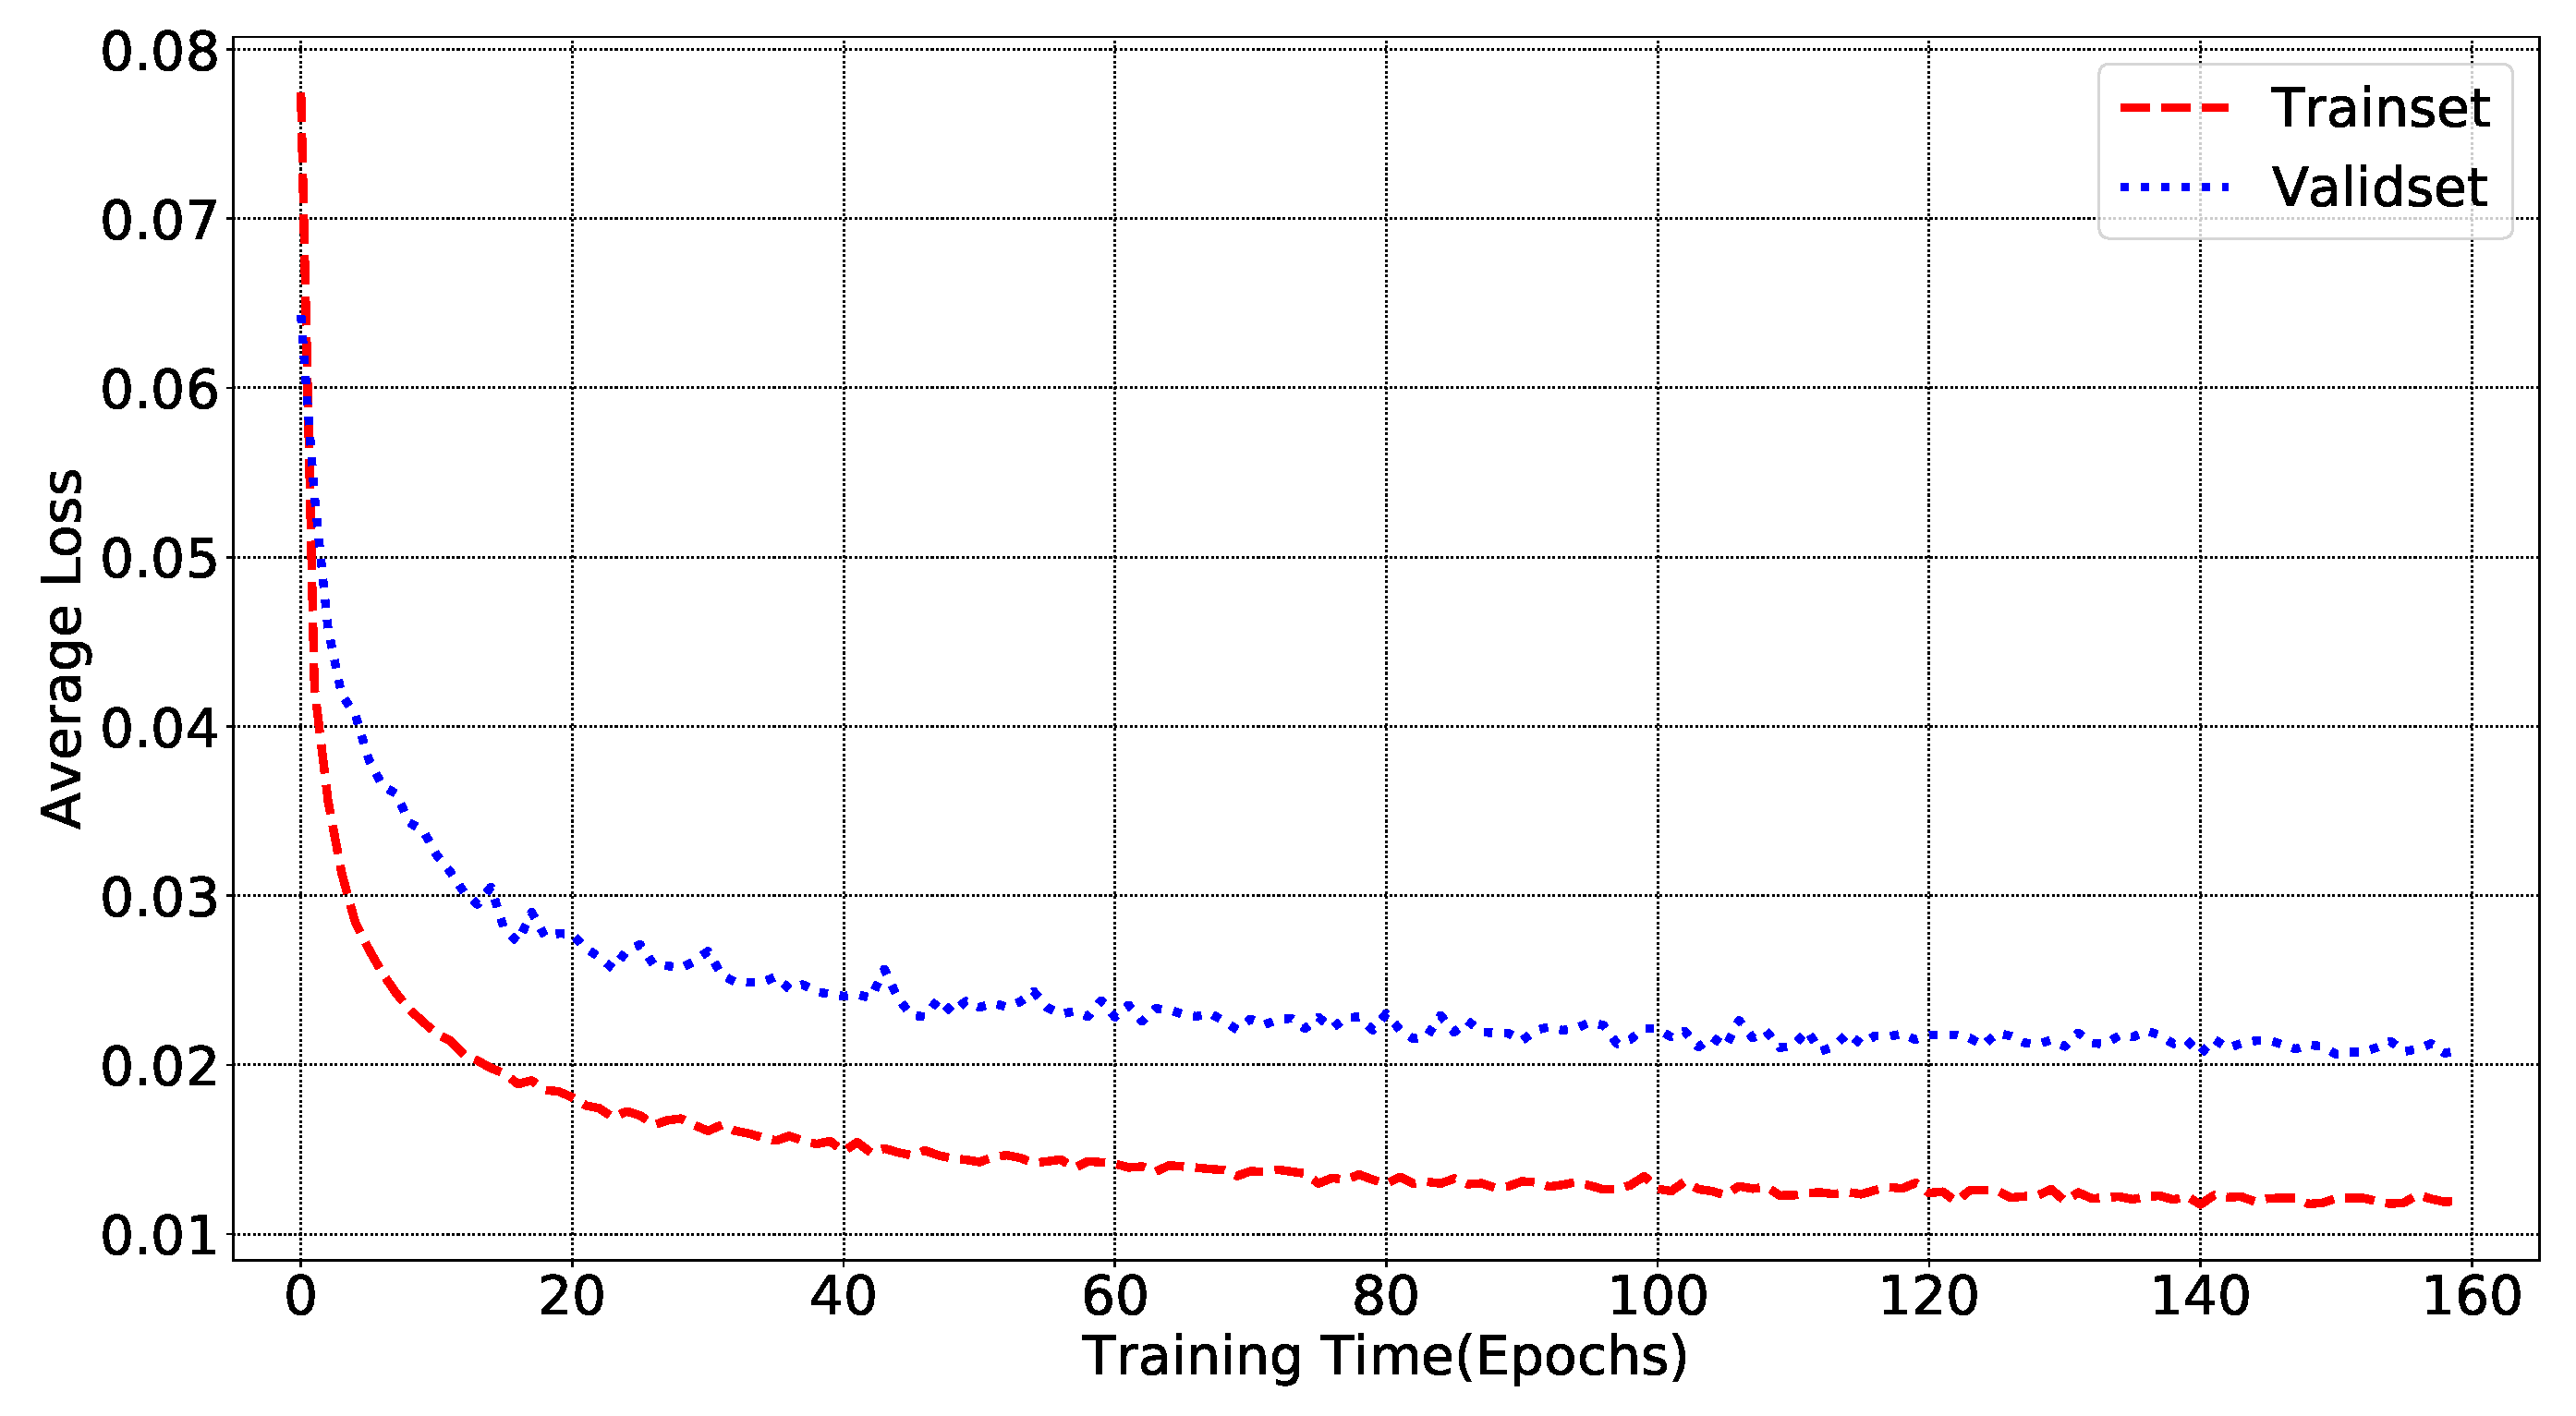
\includegraphics[width=0.48\textwidth]{figures/history.pdf}
    \caption{History of MLP's Average Loss During Cross Validation}
    \label{Fig:LossHistory}
\end{figure}

\begin{figure}[h]
    \centering
    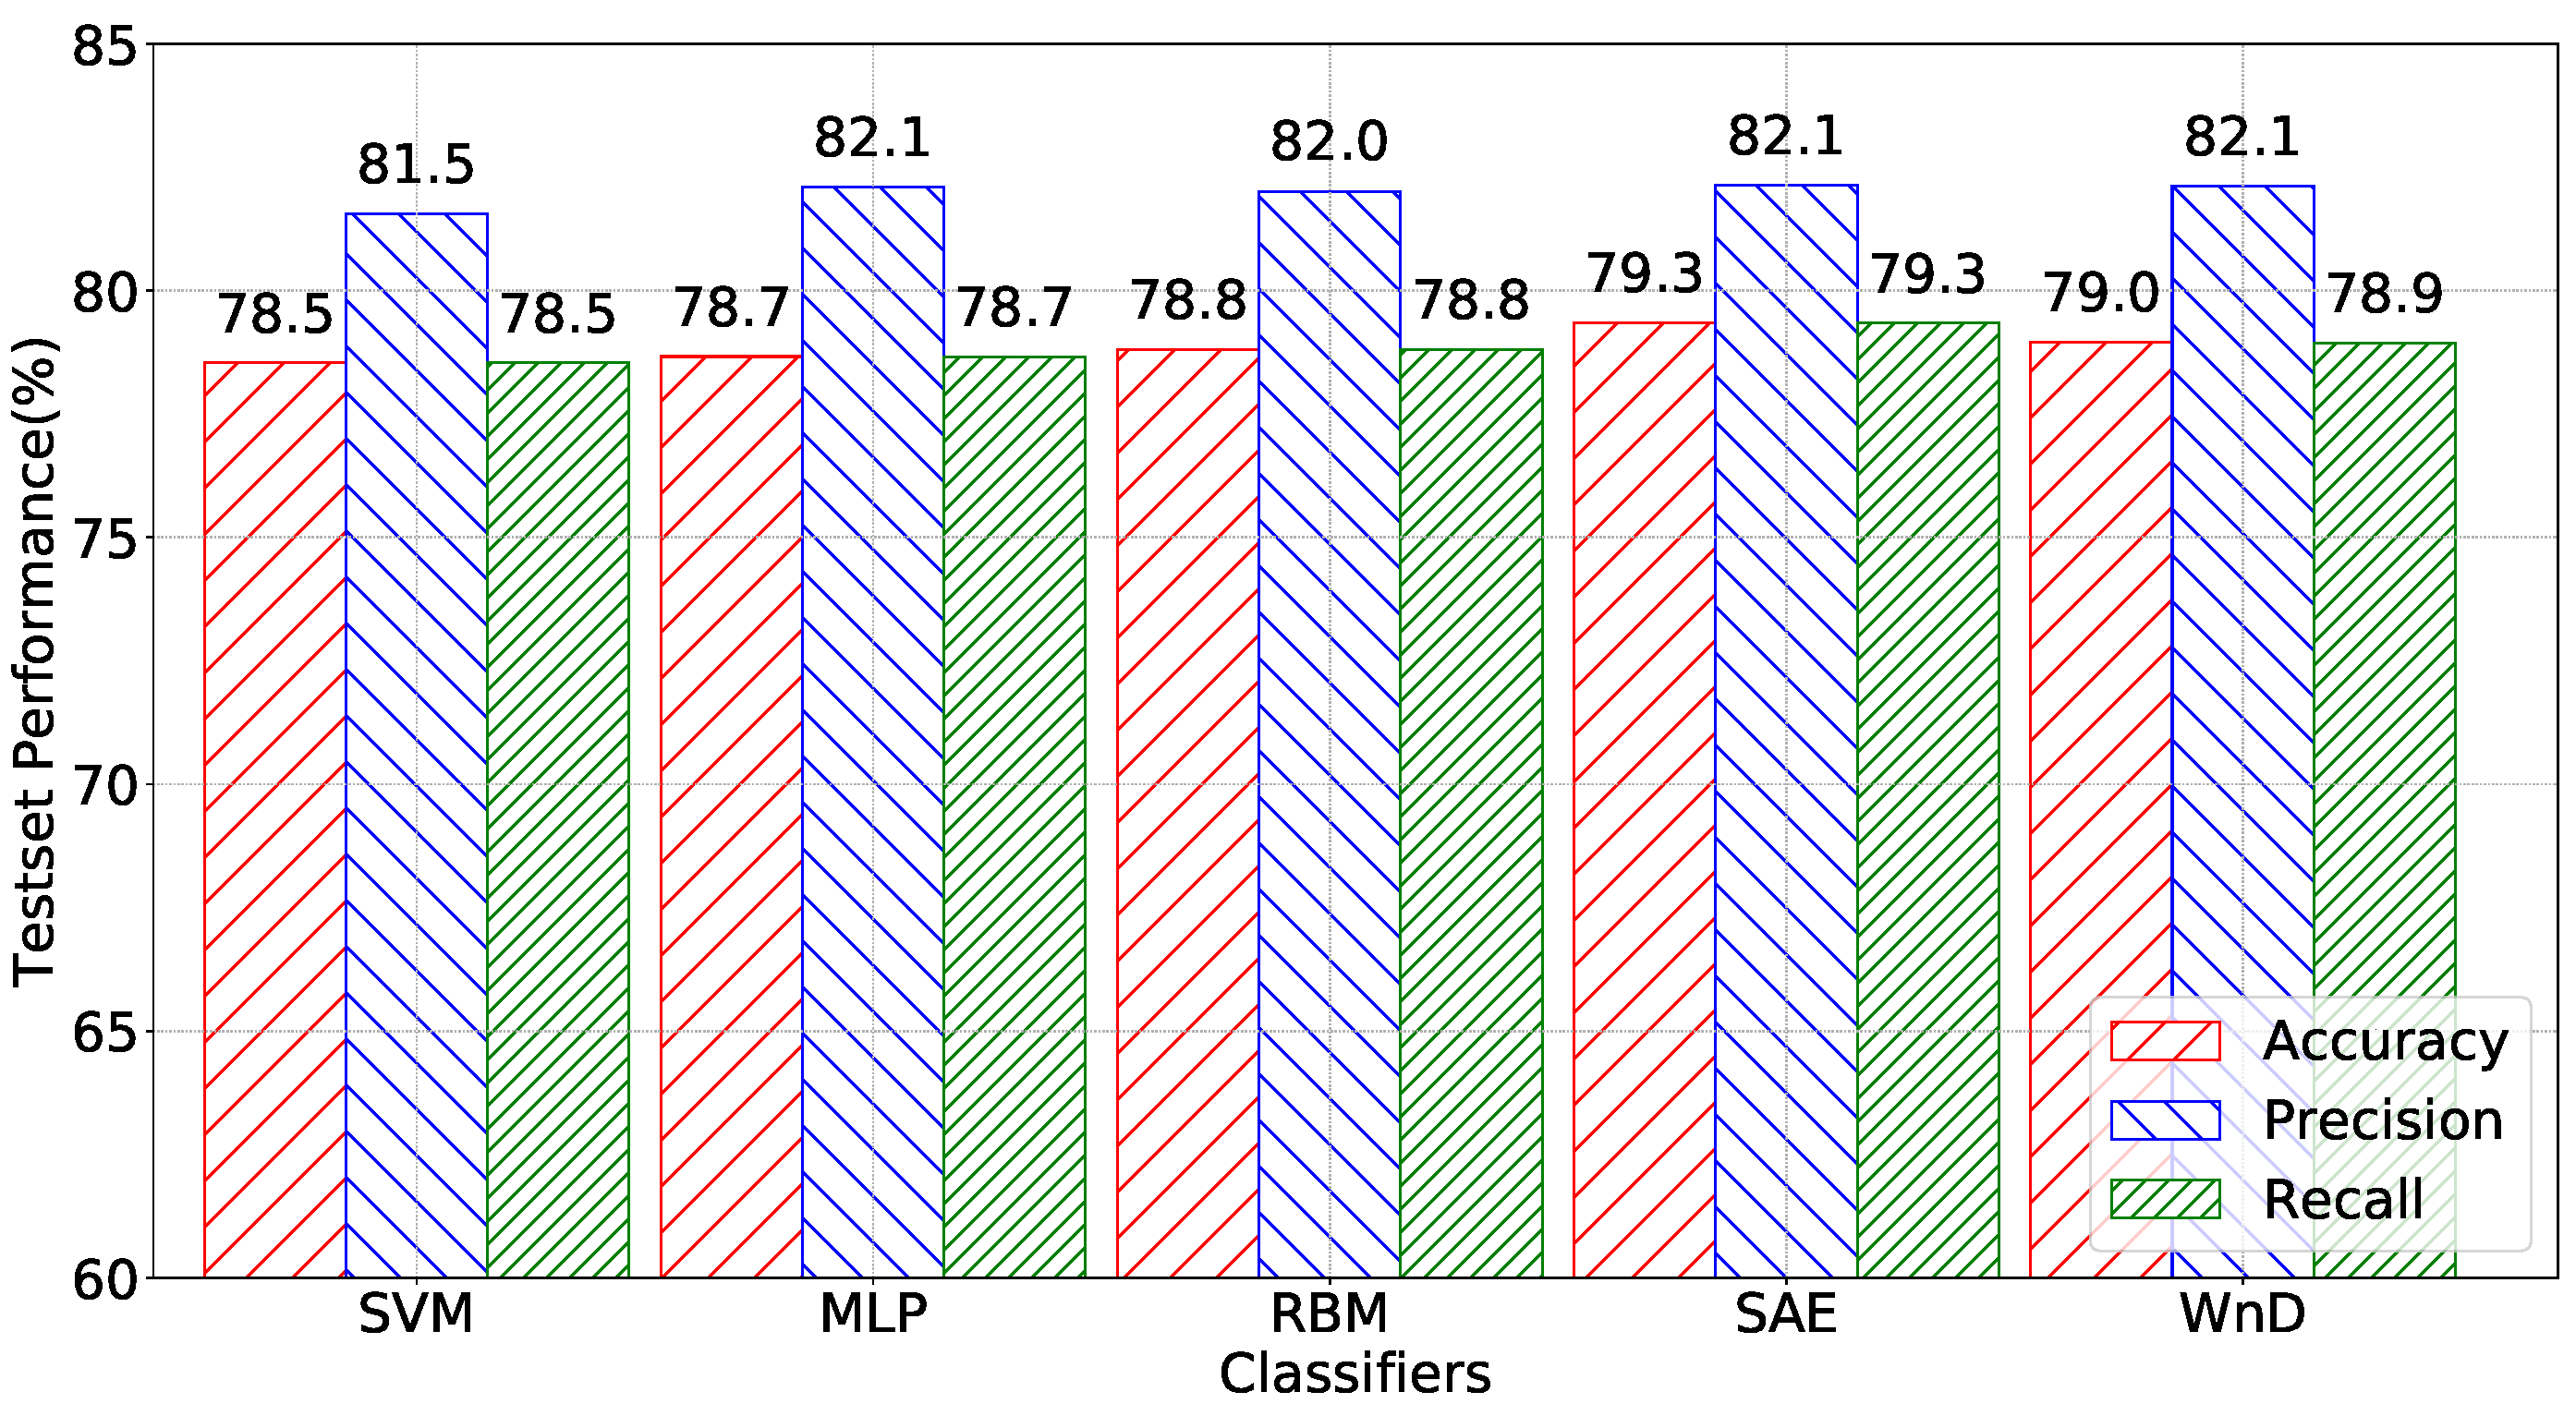
\includegraphics[width=0.48\textwidth]{figures/comp_accuracy_nsl.pdf}
    \caption{Metrics Comparison, NSL-KDD Task}
    \label{Fig:CompAccuracyNSL}
\end{figure}

\begin{figure}[h]
    \centering
    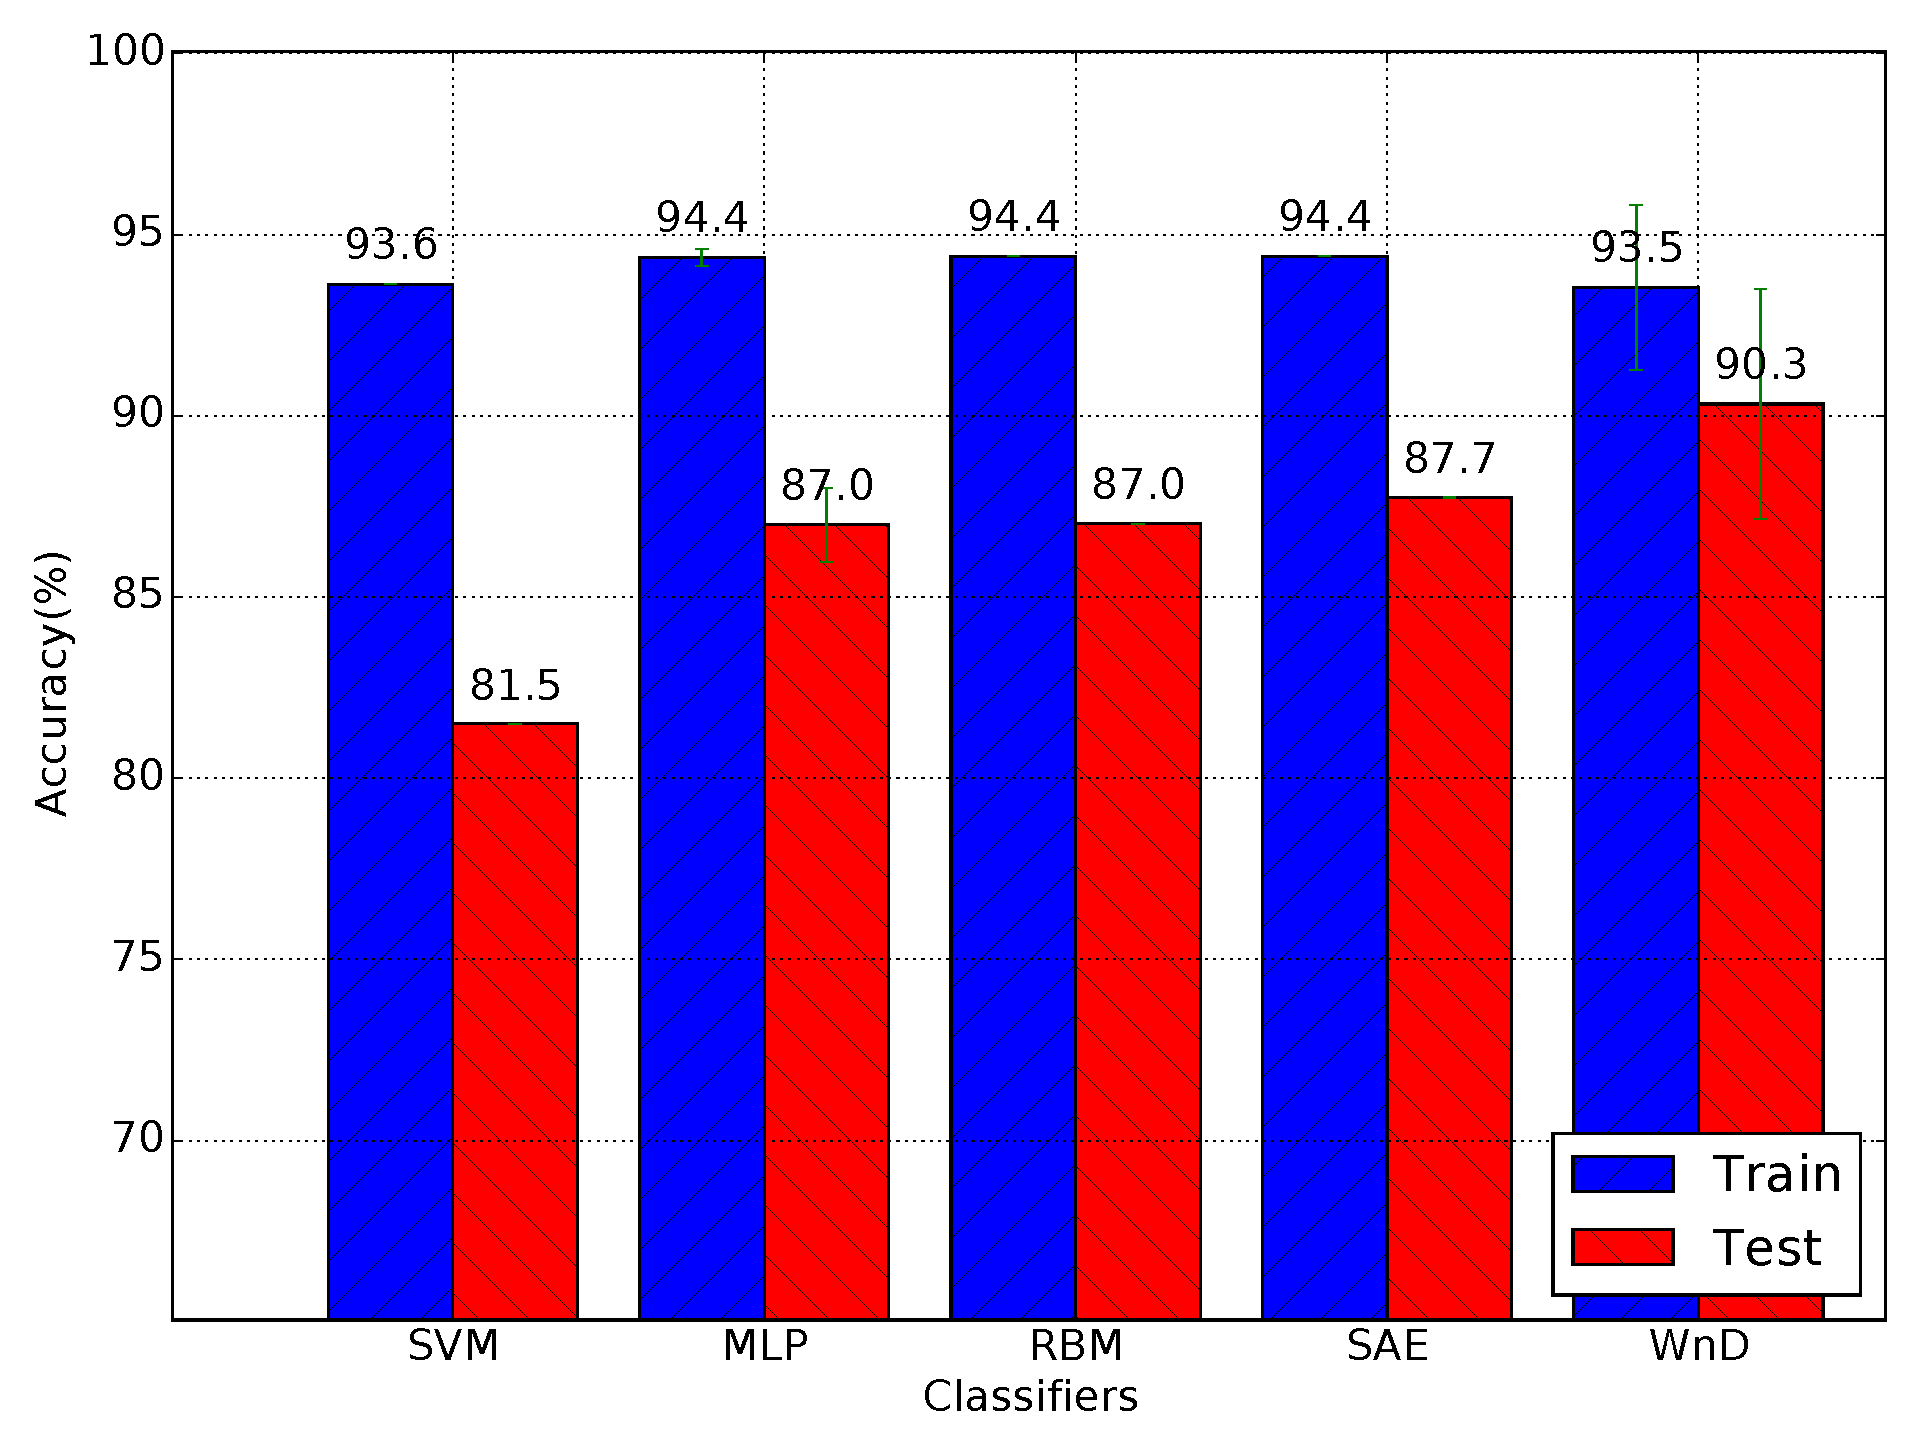
\includegraphics[width=0.48\textwidth]{figures/comp_accuracy_unsw.pdf}
    \caption{Metrics Comparison, UNSW-NB15 Task}
    \label{Fig:CompAccuracyUNSW}
\end{figure}

\begin{table}[]
    \centering
    \caption{Per-class Precision/Recall on the NSL-KDD Task}
    \label{Tab:PrecisionRecall}
    \begin{tabular}{c|c|ccccc}
        \hline
        \hline
                             &            & \multicolumn{5}{c}{Traffic Class} \\
        \cline{3-7}
                             &            & Normal & DoS   & Probe & U2R   & R2L \\
        \hline
        \multirow{2}{*}{SVM} & Precision  & 72.82  & 75.27 & 93.85 &  6.32 & 96.65 \\
        \cline{2-2}
                             & Recall     & 96.18  & 72.16 & 82.16 &  6.06 & 13.34 \\
        \hline
        \multirow{2}{*}{MLP} & Precision  & 69.18  & 95.49 & 85.58 & 59.52 & 92.01 \\
        \cline{2-2}
                             & Recall     & 96.66  & 82.31 & 69.28 &  6.31 & 15.03 \\
        \hline
        \multirow{2}{*}{RBM} & Precision  & 69.41  & 95.41 & 85.23 & 41.51 & 93.86 \\
        \cline{2-2}
                             & Recall     & 96.81  & 83.89 & 64.74 &  5.56 & 15.48 \\
        \hline
        \multirow{2}{*}{SAE} & Precision  & 70.20  & 95.63 & 84.70 & 65.00 & 87.76 \\
        \cline{2-2}
                             & Recall     & 96.92  & 83.34 & 70.56 &  3.28 & 16.29 \\
        \hline
        \multirow{2}{*}{WnD} & Precision  & 70.08  & 95.59 & 84.02 & 60.34 & 91.57 \\
        \cline{2-2}
                             & Recall     & 96.88  & 83.64 & 67.84 &  4.53 & 15.34 \\
        \hline
    \end{tabular}
\end{table}


\section{Conclusion}
We study cutting-edge deep learning models to the design of network intrusion detection systems.
%First, we briefly discuss general deep learning methodology and its potential implication on the network intrusion detection problem.
%Then we describe a set of promising deep learning models in concisely mathematical languages.
With the help of our open-source Tensorflow-based deep learning library NetLearner, we perform a comparative evaluation of those models on two network intrusion detection tasks using the NSL-KDD and UNSW-NB15 datasets. Preliminary experimental results show that for the NSL-KDD task, sparse autoencoder achieves accuracy similar to the existing machine learning solutions; for the UNSW-NB15 dataset, deep neural network models with greater generalization capability achieve better accuracy than SVM based solutions.


%
% The following two commands are all you need in the
% initial runs of your .tex file to
% produce the bibliography for the citations in your paper.
\bibliographystyle{abbrv}
\bibliography{sigproc}  % sigproc.bib is the name of the Bibliography in this case
% You must have a proper ".bib" file
%  and remember to run:
% latex bibtex latex latex
% to resolve all references
%
% ACM needs 'a single self-contained file'!
%

%\nocite{*}
%\balancecolumns % GM June 2007
% That's all folks!
\end{document}
